\documentclass[a4paper,titlepage,openright,12pt]{report}
\usepackage{graphicx}    
%\usepackage{epsfig}   
\usepackage[font=footnotesize]{subfig}
\usepackage{float}
\usepackage{fancyhdr}                              
\usepackage{makeidx}
\usepackage[nottoc,notlot,notlof]{tocbibind}     
\usepackage{supertabular}
\usepackage{array}              
\usepackage{setspace} 
\usepackage{enumerate}
\usepackage{rotating}
\usepackage{moreverb}
\usepackage{multirow}
\usepackage{amsmath}
\usepackage{amsthm}
\usepackage{amssymb}
\usepackage{captcont}
\usepackage{verbatim}
\usepackage{titlesec}
\usepackage{url}
\usepackage{hyperref}
\usepackage{lipsum}
%\usepackage[algoruled]{algorithm2e}
%\usepackage[figure,algoruled]{algorithm2e}
%\usepackage[figure,boxruled]{algorithm2e}

%\newtheorem{theorem}{Theorem}
%\newtheorem{corollary}[theorem]{Corollary}
%\newtheorem{conjecture}[theorem]{Conjecture}
%\newtheorem{lemma}[theorem]{Lemma}
%\newtheorem{proposition}[theorem]{Proposition}
%\newtheorem{definition}[theorem]{Definition}
%\newtheorem{Example}[theorem]{Example}
%\newtheorem{axiom}{Axiom}
%\newtheorem{remark}{Remark}
%\newtheorem{exercise}{Exercise}[section]
%\newtheorem{fact}[theorem]{Fact}
%\newtheorem{property}[theorem]{Property}
\setlength{\parindent}{0pt}%for paragraph spacing
\setlength{\parskip}{1ex plus 0.5ex minus 0.2ex}
\setlength{\textheight}{8.5in}
\pagestyle{fancy}
% with this we ensure that the chapter and section
% headings are in lowercase.
%\renewcommand{\bibname}{References}
\renewcommand{\chaptermark}[1]{\markboth{#1}{}}
\renewcommand{\sectionmark}[1]{\markright{\thesection\ #1}}
\fancyhf{} % delete current setting for header and footer
\fancyhead[LE,RO]{\bfseries\thepage}
\fancyhead[LO]{\bfseries\rightmark}
\fancyhead[RE]{\bfseries\leftmark}
%\rfoot{\bfseries\thepage}
\cfoot{\em $\copyright$ 2013, Indian Institute of Technology Delhi}
\renewcommand{\headrulewidth}{0.5pt}
\renewcommand{\footrulewidth}{0.5pt}
\addtolength{\headheight}{2.5pt} % make space for the rule

\fancypagestyle{plain}{%
\fancyhead{} % get rid of headers on plain pages
\fancyfoot{}
%\rfoot{\bfseries\thepage}
\cfoot{\em $\copyright$ 2013, Indian Institute of Technology Delhi}
\renewcommand{\headrulewidth}{0pt} % and the line
}

%% The smart version of cleardouble page.
\let\origdoublepage\cleardoublepage
\newcommand{\clearemptydoublepage}{%
  \clearpage
  {\pagestyle{empty}\origdoublepage}%
}

\let\cleardoublepage\clearemptydoublepage


\date{}


\addtolength{\oddsidemargin}{30pt}
\addtolength{\evensidemargin}{-40pt}

\titlespacing*{\chapter}{0pt}{-50pt}{20pt}
\titleformat{\chapter}[display]{\normalfont\huge\bfseries}{\chaptertitlename\ \thechapter}{20pt}{\Huge}
% \DeclareGraphicsExtensions{.pdf,.png,.jpg,.ps}
\floatstyle{boxed} 
\restylefloat{figure}
\setcounter{lofdepth}{2}
\setcounter{lotdepth}{2}

\newtheorem{claim}{Claim}[section]
\newtheorem{theorem}{Theorem}[section]
\newtheorem{defn}{Definition}[section]
\newtheorem{fact}{Fact}[section]

\graphicspath{{./Figures/}}
\begin{document}

%\begin{comment}
% Begin title page
\begin{titlepage}
\begin{center}

\LARGE{\textsf{\bfseries ENTER YOUR THESIS TITLE HERE}}\\
\vspace{20pt}
\normalsize
\emph{A thesis submitted in partial fulfillment} \\
\emph{of the requirements for the degree of} \\
\vspace{20pt}
\bfseries BACHELOR OF TECHNOLOGY \\
\vspace{20pt}
\emph {in}\\
\vspace{20pt}
\bfseries Computer Science \& Engineering \\
\vspace{20pt}
\emph {by}\\
\vspace{20pt}
\Large{\textsf{\bfseries ENTER YOUR NAME}} \\
{\normalsize \textsf{\bfseries Entry No. ENTRY NUMBER}}\\
\ \\
%\ \\
{\normalsize \emph {Under the guidance of}}
\ \\
\Large{\textsf{\bfseries YOUR ADVISER}} \\
\ \\
\vspace{30pt}
%\begin{center}

\includegraphics[scale=0.2]{iit_logo.pdf} \\
\vspace{10pt}
%\end{center}
\large{\textsc{Department of Computer Science and Engineering,\\
Indian Institute of Technology Delhi.\\ May 2013.}}
\end{center}
\end{titlepage}

%\newpage
%\cleardoublepage
\onehalfspacing
\thispagestyle{empty}

\normalfont
\begin{center}
\LARGE{ Certificate} 
\end{center}

\vspace{0.5in}

This is to certify that the thesis titled {\bfseries DATA ANALYSIS OF COMMODITY PRICES} being submitted by
{\bfseries KAPIL THAKKAR} for the award of {\bfseries Master of Technology} in {\bfseries Computer Science \& Engineering} is a record of bona fide work carried out by him under my guidance and supervision at the {\bfseries Department of Computer Science \& Engineering}. The work presented in this thesis has not been submitted elsewhere either in part or full, for the award of any other degree or diploma.

\vspace{1.5in}


{\bfseries Dr. Aaditeshwar Seth} \\
{\bfseries Department of Computer Science and Engineering} \\
{\bfseries Indian Institute of Technology, Delhi}\\ 

\thispagestyle{empty}
%\begin{center}
\LARGE{Acknowledgments} 
\end{center}

\vspace{0.5in}

%Replace \lipsum with your acknowledgement
\lipsum[1]

\vspace{1.5in}

{\bfseries YOUR NAME}

\thispagestyle{empty}


% \setcounter{page}{1}
% \pagenumbering{roman}
\thispagestyle{empty}
\begin{center}
\LARGE{Abstract}
\end{center}

\vspace{0.5in}


Supply demand imbalance, natural calamities etc. may not always be the reason behind the rise in the price of a commodity. It may be a result of artificial supply deficit planned intelligently by traders’ nexus to earn more profits through manipulation of supply of commodity and hence indirectly controlling their prices. Our attempt is to locate such hikes in prices which seem suspicious (we call them anomalies). We try to detect such anomalies by stating some hypothesis first and then algorithmically try to find the time-line during which it violates the stated hypothesis.


\thispagestyle{empty}
\begin{center}
\LARGE{Acknowledgments} 
\end{center}

\vspace{0.5in}

%Replace \lipsum with your acknowledgement
\lipsum[1]

\vspace{1.5in}

{\bfseries YOUR NAME}


\thispagestyle{empty}
\tableofcontents

\thispagestyle{empty}

\listoffigures

\listoftables
%\end{comment}

\thispagestyle{empty}
\cleardoublepage
\onehalfspacing
%%%%%%%%%%%%%%%%%%%%%%%%%%%%%%%%%%%%%%%%%%%%%%%%%%%%%%%%%%%%
 
\setcounter{page}{1}
\pagenumbering{arabic}

%You may have as many chapters as you please. This is just for reference.

\chapter{Introduction}

%Replace \lipsum with text.
% You may have as many sections as you please. This is just for reference.

\section{Objective}

Our objective is to create library with some set of functionalities to detect anomalies in the give input time series​. Anomalies will be based on the hypothesis stated by the user​. For particular scenario stated by user, execute appropriate algorithms and report the anomalies in the time series.

%You should cite papers in the following manner: Bayliss et al.~\cite{Bay1} gave an iterative method for Helmholtz equation etc.
%Similar work has been done in \cite{Bailey,Ernst,Gold3}.


\section{Motivation}

Supply demand imbalance, natural calamities etc. may not always be the reason behind the rise in the price of a commodity. ​It may be a consequence of artificial supply deficit planned intelligently by traders’ nexus for profiteering through manipulation of supply of commodity and hence indirectly controlling their prices. ​Our attempt is to locate such hikes in prices which seem suspicious (we call them anomalies).​ To detect and analyse the characteristics of anomalies in the prices of commodities. Currently we have considered the case of onion and based on that we are looking forward to develop library for any time-series.

\section{Related Work}

Supply demand imbalance, natural calamities etc. may not always be the reason behind the rise in the price of a commodity. ​It may be a consequence of artificial supply deficit planned intelligently by traders’ nexus for profiteering through manipulation of supply of commodity and hence indirectly controlling their prices. ​Our attempt is to locate such hikes in prices which seem suspicious (we call them anomalies).​ To detect and analyse the characteristics of anomalies in the prices of commodities. Currently we have considered the case of onion and based on that we are looking forward to develop library for any time-series.


% You may add figures in the following manner.
\begin{figure}[here]
\begin{center}	
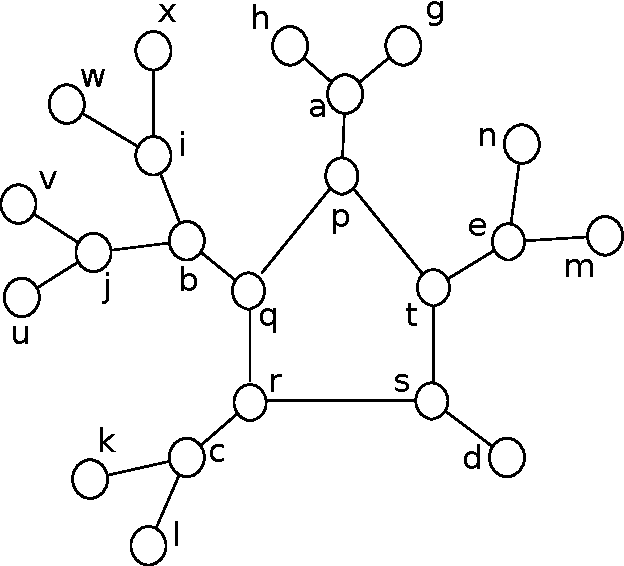
\includegraphics[scale=0.4]{pent} 
\caption{Pentagon $pqrst$}
\label{fig:pent}
\end{center}
\end{figure}

\lipsum[1]

\section{SECTION NAME}
\lipsum[2]

\begin{table}
\centering
\begin{tabular}{| c | c |}
\hline
{\bf item 1} & {\bf item 2} \\ \hline
%
abcde & 5 \\ \hline
%
pqrst & 4 \\ \hline
\end{tabular}
\caption{A sample table}
\label{table:1}
\end{table}


\chapter{CHAPTER NAME}

%Replace \lipsum with text.
% You may have as many sections as you please. This is just for reference.

\section{SECTION NAME}
\lipsum[2]

\section{SECTION NAME}
\lipsum[3]

\section{SECTION NAME}
\lipsum[2]

\chapter{Study of Onion Data: Collection and Analysis}


\section{System}

For now, we are only working over onion data. We have three actors in model: Farmers who are producers of onion, traders who are collectively responsible for supply of onions across countries and consumers who purchase onions.

\begin{figure}[here]
\begin{center}	
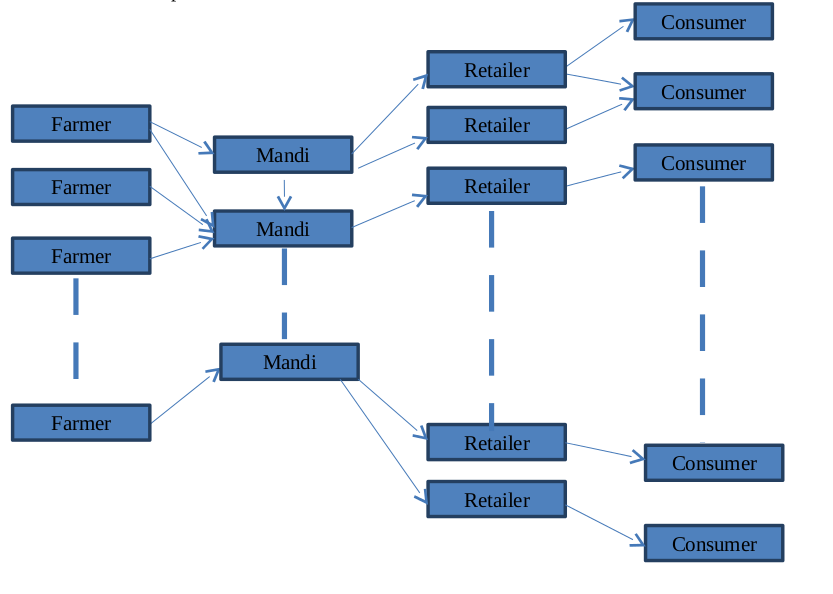
\includegraphics[scale=0.4]{3_1} 
\caption{Normal Supply Chain}
\label{fig:Normal Supply Chain}
\end{center}
\end{figure}

Farmers sell their produce to traders in nearest mandi offering better price. These traders sell these commodities to traders in other mandis or to retailers. Consumers purchase commodities for consumption from one of the retail stores. This way commodity reaches consumers from farmers following a huge chain of traders and retailers.

Under APMC act, mandis were established at different places across country so that farmers can sell their produce directly in mandi and get good returns (wholesale price). There are around 1500 mandis located in different places across country which log their daily arrival of onion, minimum, maximum, modal selling price per quintal of onion data to AGMARKNET. Retailers purchase from these mandis and sell to end customers at retail price. There are around 70+ centres across country which maintains retail price of onion on Ministry of consumer affairs website.

\section{Data we have}

We have following data:

\begin{enumerate}

\item Daily wholesale price of onion for 1514 mandis 
\item Daily arrival of onion information for 1514 mandis
\item Daily retail price of onion for 76 centres
\item Dates and location for hoarding reports from news articles
\item Longitude and latitude of mandis and centres

\end{enumerate}

Onion Data was collected from the the government websites,\cite{agmarknet} for arrival and wholesale price data and \cite{retailpricecollection} (Department of Consumer Affairs) for retail price data. Crawlers were written to collect the data from these datewise for the period of approximately 9.5 years, starting from Jan 2006 to Jun 2015. More data can be added simply by running crawlers again.


\section{Normal market behaviour}

\begin{enumerate}

\item Wholesale price is inversely proportional to arrival of commodity –higher production of crop will lead to more and more crop hitting market for sell. Hence more arrival which will result in surplus supply leading to drop in wholesale prices.

\item  Retail price is directly proportional to wholesale price – commodities reach customers through a long chain of traders and retailers, adding value at every stage of chain. So, retail price at which customers purchase commodities are more than wholesale.

\end{enumerate}

Any divergence from these characteristics of normal market leads to suspicious price hike situations/anomalies.


\section{What are the reasons for anomaly?}

Primarily there are 3 main reasons of anomaly.

\begin{enumerate}

\item \textbf{Government Policies:} When the price is low in the country, still government allows the export of onion in large amount, or supports it by keeping low minimum price then the prices can rise up drastically.

\item \textbf{Unseasonal Rainfall:} Due to insufficient rainfall, heavy rainfall or unseasonal rainfall, onion crop may get affected and the produce is low and wholesale price may rise up. But, this reason still is validating that wholesale price is inversely proportional to arrival, it may be just prices will be little higher than it was supposed to be.

\item \textbf{Hoarding:} When traders/wholesalers store the onion and does not release the stock in the market in the expectation of the good prices in the future, it will create the artificial deficit in the market and will shoot up the onion prices in the retail market due to low arrival in the retail market. The reason people do this is to expect the higher prices in the time of low production or may be for security. For example, if it is expected that this year the rainfall will be very low, then people may think that, due to that, production will be low in the future and so they will start storing onion right now and that will also create deficit in the market and price will go up. 

\end{enumerate}

So our study will focus on detection of anomalies in data and if possible comment on the possible reason for the anomaly.

\section{Mapping of wholesale price to retail price}

Voronoi Diagram is used to map every mandi to nearest possible centre. The centres with retail data were considered fixed points and country was divided into 76 regions. All the mandis falling in that region are mapped to the respective centre.


\begin{figure}[here]
\begin{center}	
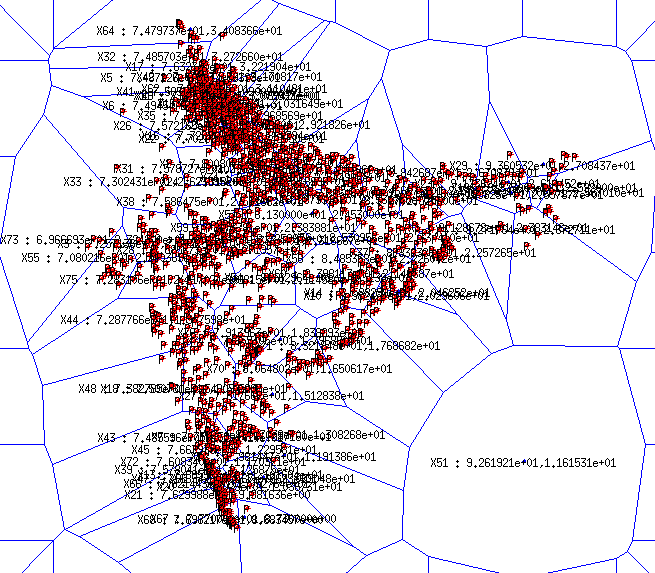
\includegraphics[scale=0.7]{3_2} 
\caption{Voronoi Diagram}
\label{fig:Voronoi Diagram}
\end{center}
\end{figure}


After all the mandis are mapped to their nearest centre, wholesale and arrival at every centre is computed. Wholesale price at centre is average of modal price of all mandis in its region and arrival was computed as the sum of the arrival at the mandis in its region. While calculating the wholesale price, the distance between centre and the mandi was not considered.

Corresponding to every date and location of hoarding news report, values like current year arrival, last year arrival, Percentage difference in wholesale- retail etc. were computed. Following table resulted from these computations.


\section{How to Define Anomaly?}

To answer this question, we went through the series of the news articles when the hoarding is in the news. Then looking over those articles, we try to see that why they are reporting to news, what happened so that people are giving it name of hoarding and how reporters are making conclusion that it may be the class of the hoarding.



\chapter{CHAPTER NAME}

%Replace \lipsum with text.
% You may have as many sections as you please. This is just for reference.

\section{SECTION NAME}
\lipsum[2]

\section{SECTION NAME}
\lipsum[3]

\section{SECTION NAME}
\lipsum[2]

\chapter{Conclusion}

\lipsum[2]

\bibliographystyle{plain}
\bibliography{biblio}

%\appendix
%\chapter{CHAPTER NAME}

\section{SECTION NAME}
\lipsum[1]

\section{SECTION NAME}
\lipsum[2]

\end{document}
	